% LaTeX mintafájl szakdolgozat és diplomamunkáknak az
% SZTE Informatikai Tanszékcsoportja által megkövetelt
% formai követelményeinek megvalósításához
% Modosítva: 2011.04.28 Nemeth L. Zoltan
% A fájl használatához szükséges a magyar.ldf 2005/05/12 v1.5-ös vagy későbbi verziója
% ez letölthető a http://www.math.bme.hu/latex/ weblapról, a magyar nyelvű szedéshez
% Hasznos információk, linekek, LaTeX leírások a www.latex.lap.hu weboldalon vannak.
%

\documentclass[12pt]{report}

%Magyar nyelvi támogatás (Babel 3.7 vagy későbbi kell!)
\def\magyarOptions{defaults=hu-min}
\usepackage[magyar]{babel}

%Az ékezetes betűk használatához:
\usepackage{t1enc}% ékezetes szavak automatikus elválasztásához
\usepackage[utf8]{inputenc}% ékezetes szavak beviteléhez

% A formai kovetelmenyekben megkövetelt Times betűtípus használata:
\usepackage{times}

%Az AMS csomagjai
\usepackage{amsmath}
\usepackage{amssymb}
\usepackage{amsthm}

%A fejléc láblécek kialakításához:
\usepackage{fancyhdr}

%Természetesen további csomagok is használhatók,
%például ábrák beillesztéséhez a graphix és a psfrag,
%ha nincs rájuk szükség természetesen kihagyhatók.
\usepackage{graphicx}
\usepackage{psfrag}

\usepackage{setspace}

\usepackage{hyperref}
\hypersetup{
    colorlinks,
    citecolor=black,
    filecolor=black,
    linkcolor=black,
    urlcolor=black
}

\usepackage{cite}

%\usepackage{enumitem}
\usepackage{enumerate}

% Színek
\usepackage{color}
\definecolor{myCommentColorGreen}{RGB}{0,128,0}
\definecolor{myLineNumberGray}{RGB}{128,128,128}

% Forráskódhoz
\usepackage{listings}
\lstset{ %
    %backgroundcolor=\color{white},   % choose the background color; you must add  \usepackage{color} or \usepackage{xcolor}
    basicstyle=\scriptsize, %\footnotesize,         % the size of the fonts that are used for    the code
    %breakatwhitespace=false,         % sets if automatic breaks should only      happen at whitespace
    breaklines=true,                  % sets automatic line breaking
    captionpos=b,                    % sets the caption-position to          bottom
    commentstyle=\color{myCommentColorGreen},    % comment style
    %deletekeywords={...},            % if you want to delete keywords              from the given language
    %escapeinside={\%*}{*)},          % if you want to add LaTeX                within your code
    %extendedchars=true,              % lets you use non-ASCII                  characters; for 8-bits encodings only, does not work with                  UTF-8
    frame=leftline,                   % adds a frame around the                    code
    %keepspaces=true,                 % keeps spaces in text,                      useful for keeping indentation of code (possibly needs                      columns=flexible)
    inputpath=../../../code/gepard,
    keywordstyle=\color{blue},        % keyword style
    language=C++,                     % the language of                          the code
    literate=%
        {á}{{\'a}}1
        {é}{{\'e}}1
        {í}{{\'i}}1
        {ó}{{\'o}}1
        {ö}{{\"o}}1
        {ő}{{\H{o}}}1
        {ú}{{\'u}}1
        {ü}{{\"u}}1
        {ű}{{\H{u}}}1
        {Á}{{\'A}}1
        {É}{{\'E}}1
        {Í}{{\'I}}1
        {Ó}{{\'O}}1
        {Ö}{{\"O}}1
        {Ő}{{\H{O}}}1
        {Ú}{{\'U}}1
        {Ü}{{\"U}}1
        {Ű}{{\H{U}}}1,
    %morekeywords={*,...},            % if you want to                            add more keywords to the set
    numberfirstline=true,
    numbers=left,                     % where to put                              the line-numbers; possible values are (none, left, right)
    numbersep=10pt,                   % how far theline-numbers are from the code
    numberstyle=\tiny\color{myLineNumberGray}, % the stylethat is used for the line-numbers
    %name=\thelstnumber,              %
    %rulecolor=\color{black},         % if notset, the frame-color may be changed online-breaks within not-black text (e.g.comments (green here))
    %showspaces=false,                % showspaces everywhere adding particularunderscores; it overrides'showstringspaces'
    %showstringspaces=false,          % underline spaces within strings only
    %showtabs=false,                  % show tabs within strings addingparticular underscores
    %stepnumber=2,                    % the step between two line-numbers.If it's 1, each line will benumbered
    %stringstyle=\color{mymauve},     % string literal style
    tabsize=4,                        % sets default tabsize to 2    spaces
    %title=\lstname                   % show the filename of     files included with     \lstinputlisting; also try     caption instead of title
}

% Kép mellett folyó íráshoz
\usepackage{wrapfig}

\usepackage[labelfont=it,justification=centering]{caption}

\usepackage{graphicx}
\usepackage{epigraph}
%\epigraphfontsize{\small\itshape}

%Tételszerű környezetek definiálhatók, ezek most fejezetenként együtt számozódnak, pl.
\newtheorem{tét}{Tétel}[chapter]
\newtheorem{defi}[tét]{Definíció}
\newtheorem{lemma}[tét]{Lemma}
\newtheorem{áll}[tét]{Állítás}
\newtheorem{köv}[tét]{Következmény}

%Ha a megjegyzések és a példak szövegét nem akarjuk dőlten szedni, akkor
%az alábbi parancs után kell őket definiální:
\theoremstyle{definition}
\newtheorem{megj}[tét]{Megjegyzés}
\newtheorem{pld}[tét]{Példa}

%%% Saját parancsok
% Az angol kifejezések kiemelése
\newcommand{\inenglish}[1]{\textsl{#1}}
\newcommand{\inenglishfn}[1]{\footnotesize{\inenglish{#1}}}

%\hyphenation{sza-bály el-kü-lö-ní-tett}

%Margók:
\hoffset -1in
\voffset -1in
\oddsidemargin 35mm
\textwidth 150mm
\topmargin 15mm
\headheight 10mm
\headsep 5mm
\textheight 237mm

\begin{document}


%%%%%%%%%%%%%%%%%%%%%%%%%%%%%%%%%%%%%%%%%%%%%%%%%%%%%%%%%%%%%%%%%%%%%%
%%   Címlap                                                         %%
%%%%%%%%%%%%%%%%%%%%%%%%%%%%%%%%%%%%%%%%%%%%%%%%%%%%%%%%%%%%%%%%%%%%%%

    %A FEJEZETEK KEZDŐOLDALAINAK FEJ ÉS LÁBLÉCE:
    %a plain oldalstílust kell átdefiniálni, hogy ott ne legyen fejléc:
    \fancypagestyle{plain}{%
    %ez mindent töröl:
    \fancyhf{}
    % a láblécbe jobboldalra kerüljön az oldalszám:
    \fancyfoot[R]{\thepage}
    %elválasztó vonal sem kell:
    \renewcommand{\headrulewidth}{0pt}
    }

    %A TÖBBI OLDAL FEJ ÉS LÁBLÉCE:
    \pagestyle{fancy}
    \fancyhf{}
    \fancyhead[L]{OpenGL-ES 2.0 alapú Path API}
    \fancyfoot[R]{\thepage}


    %A címoldalra se fej- se lábléc nem kell:
    \thispagestyle{empty}

    \begin{center}
    \vspace*{1cm}
    {\Large\bf Szegedi Tudományegyetem}

    \vspace{0.5cm}

    {\Large\bf Informatikai Tanszékcsoport}

    \vspace*{3.8cm}

    % Tíz sorral fentebb is át kell írni!!!
    {\LARGE\bf OpenGL-ES 2.0 alapú Path API}


    \vspace*{3.6cm}

    {\Large Diplomamunka}
    % vagy {\Large Szakdolgozat}

    \vspace*{4cm}

    %Értelemszerűen megváltoztatandó:
    {\large
    \begin{tabular}{c@{\hspace{4cm}}c}
    \emph{Készítette:}     &\emph{Témavezető:}\\
    \bf{Ledán Szilárd}  &\bf{Dr. Kiss Ákos}\\
    informatika szakos     & adjunktus\\
    hallgató &
    \end{tabular}
    }

    \vspace*{2.3cm}

    {\Large
    Szeged
    \\
    \vspace{2mm}
    2016
    }
    \end{center}


    % 1.5-ös sorköz:
    % ezt javasolják:  \linespread{1.25}
    % és ez bevált, de ehhez kellett a \usepackage{setspace} csomag betöltése.
    \onehalfspacing


%%%%%%%%%%%%%%%%%%%%%%%%%%%%%%%%%%%%%%%%%%%%%%%%%%%%%%%%%%%%%%%%%%%%%%
%%   Mottó                                                          %%
%%%%%%%%%%%%%%%%%%%%%%%%%%%%%%%%%%%%%%%%%%%%%%%%%%%%%%%%%%%%%%%%%%%%%%

    \clearpage
    \thispagestyle{empty}
    {
    \setlength\epigraphrule{0pt}
    \linespread{1.0}\epigraph{\small\emph{,,A világ csak híd, menj át rajta,
    de ne építs rajta házat."}}{\small(IHS)}
    }


%%%%%%%%%%%%%%%%%%%%%%%%%%%%%%%%%%%%%%%%%%%%%%%%%%%%%%%%%%%%%%%%%%%%%%
%%   Tartalomjegyzék                                                %%
%%%%%%%%%%%%%%%%%%%%%%%%%%%%%%%%%%%%%%%%%%%%%%%%%%%%%%%%%%%%%%%%%%%%%%

    \tableofcontents


%%%%%%%%%%%%%%%%%%%%%%%%%%%%%%%%%%%%%%%%%%%%%%%%%%%%%%%%%%%%%%%%%%%%%%
%%   Feladatkiírás                                                  %%
%%%%%%%%%%%%%%%%%%%%%%%%%%%%%%%%%%%%%%%%%%%%%%%%%%%%%%%%%%%%%%%%%%%%%%


    %A \chapter* parancs nem ad a fejezetnek sorszámot
    \chapter*{Feladatkiírás}
    %A tartalomjegyzékben mégis szerepeltetni kell, mint szakasz(section) szerepeljen:
    \addcontentsline{toc}{section}{Feladatkiírás}

A témavezető által megfogalmazott feladatkiírás. Önálló oldalon szerepel.


%%%%%%%%%%%%%%%%%%%%%%%%%%%%%%%%%%%%%%%%%%%%%%%%%%%%%%%%%%%%%%%%%%%%%%
%%   Tartalmi összefoglaló                                          %%
%%%%%%%%%%%%%%%%%%%%%%%%%%%%%%%%%%%%%%%%%%%%%%%%%%%%%%%%%%%%%%%%%%%%%%

    \chapter*{Tartalmi összefoglaló}
    \addcontentsline{toc}{section}{Tartalmi összefoglaló}

%A tartalmi összefoglalónak tartalmaznia kell (rövid, legfeljebb egy oldalas, összefüggő megfogalmazásban)
%a következőket: a téma megnevezése, a megadott feladat megfogalmazása - a feladatkiíráshoz viszonyítva-,
%a megoldási mód, az alkalmazott eszközök, módszerek, az elért eredmények, kulcsszavak (4-6 darab).

%Az összefoglaló nyelvének meg kell egyeznie a dolgozat nyelvével. Ha a dolgozat idegen nyelven készül,
%magyar nyelvű tartalmi összefoglaló készítése is kötelező (külön lapon), melynek terjedelmét a TVSZ szabályozza.

    \subsubsection*{A téma megnevezése}

  A \emph{W3C} (World Wide Web Consortium) által \emph{Canvas 2D
Context} néven 2015-ben elfogadott ajánlás \emph{path} részének
megvalósítása \emph{OpenGL-ES 2.0} alapokon.

    \subsubsection*{A megadott feladat megfogalmazása}

  Az előbb említett \emph{Canvas} egy grafikus API~\footnote{Az
alkalmazásprogramozási felület/interfész (Application Programming Interface)
kifejezésre a továbbiakban mint \emph{API} hivatkozunk.}.
  Ez az API több grafikus függvényt definiál (ld. később).
  Jelen dolgozat témája ezek közül az úgynevezett \emph{path} részének
leprogramozása~úgy, hogy a lehető legtöbb feladatot a grafikus processzor
(\textit{GPU}) lássa el.

    \subsubsection*{A megoldásmód}

  Több megoldás közül (ld. a Háttér részt) mi az alakzatok trapézokra
bontását választottuk. Hiszen minden trapéz felbontható további két
háromszögre, mely megkötésre a GLES2 grafikus renderelő~\footnote{Az
előállítás--megjelenítés (\emph{rendering}) kifejezésre a továbbiakban
\emph{renderelés}ként hívatkozunk.} API miatt van szükség.

    \subsubsection*{Alkalmazott eszközök, módszerek}

  Az API \emph{c++11} programozási nyelven készült, használva a következő
eszközöket, technológiákat: \emph{gcc}, \emph{git}, \textit{OpenGL~ES~2.0}, \emph{\LaTeX},

    \subsubsection*{Elért eredmények}

    \subsubsection*{Kulcsszavak}

grafika, path, canvas-2D-context, OpenGL-ES 2.0


%%%%%%%%%%%%%%%%%%%%%%%%%%%%%%%%%%%%%%%%%%%%%%%%%%%%%%%%%%%%%%%%%%%%%%
%%   Bevezetés                                                      %%
%%%%%%%%%%%%%%%%%%%%%%%%%%%%%%%%%%%%%%%%%%%%%%%%%%%%%%%%%%%%%%%%%%%%%%

    \chapter*{Bevezetés}
    \label{Bevezetés}
    \addcontentsline{toc}{section}{Bevezetés}

  A környezetünkben található számítástechnikai eszközök
legtöbbjének van grafikus kijelzője, és ezen eszközök mindegyike használ
valamilyen megjelenítő~\footnote{A számítógépes grafikában egy modell
megjelenítését végző folyamatot \emph{renderelés}nek (\inenglishfn{rendering}),
a renderelést végző programrészt pedig \emph{motor}nak (\inenglishfn{engine})
hívnak} (a továbbiakban renderelő) függvénykönyvtárat. Ilyen például a Skia, a
Cairo, az OpenGL, és ilyen kíván lenni a \emph{Gepard} is. A cél egy
\emph{C++11}-es nyelven írt és több (\mbox{OpenGL~ES~2.0
\cite{Munshi:2008:OEP:1481069}}, Vulkan) grafikus renderelő motort támogató
függvénykönyvtár.

  A tervek szerint idővel a Gepard több interfésszel is rendelkezik.
Így alkot majd egy komplex grafikus alkalmazásprogramozási felületet
(\inenglish{Application Programming Interface}, a továbbiakban API). Az elsőnek
választott ilyen ismertebb interfész amit támogatni kíván az a \emph{W3C} által
készített \emph{Canvas 2D Context}~\cite{Cabanier:14:HCC} előírás.

  A \emph{Canvas 2D Context} (a továbbiakban \emph{Canvas}) előírás
2015-ös kiadása több elkülönített részből állítja össze az API-t. Ezen részek
egyike az úgynevezett \emph{Path}. Az említett 2015-ös előírás az 5., 8. és 11.
fejezetekben részletezi a Path-szal szembeni elvárásokat. A Path maga a
definiált grafikus alakzatokhoz képest bonyolultabbak leírását biztosító
eszköz. A Háttér (\ref{Háttér}.) fejezetben részletesebben kifejtjük a path-t
építő eszköz lehetőségeit és szabályait. Itt most csak annyiban kell kitérjünk
rá, hogy alapvetően két nagyobb részből áll. A \emph{körvonalból}
(\inenglish{stroke}) és a \emph{kitöltésből} (\inenglish{fill}).

  Jelen dolgozat az említett \emph{Path} rész megvalósítását kívánja bemutatni.
Azt, hogy milyen szabályoknak kellett megfelelni, illetve milyen lehetőségeket
biztosított a választott OpenGL~ES~2.0 (a továbbiakban GLES2) szabvány, és azt,
hogy hogyan alkot köztes réteget ezek között a Gepard Path-t rajzoló, renderelő
része.

  Első körben nem volt cél a ,,leggyorsabban futó'' és ,,legkisebb méretű''
Path-t rajzoló API elkészítése. Célunk egy lehetséges megvalósítás megtalálása,
és ez alapján egy olyan eszköz megalkotása volt, amely képes a választott
előírás (Canvas) elvárásait teljesíteni.


%%%%%%%%%%%%%%%%%%%%%%%%%%%%%%%%%%%%%%%%%%%%%%%%%%%%%%%%%%%%%%%%%%%%%%
%%   Háttér                                                         %%
%%%%%%%%%%%%%%%%%%%%%%%%%%%%%%%%%%%%%%%%%%%%%%%%%%%%%%%%%%%%%%%%%%%%%%

    \chapter{Háttér}
    \label{Háttér}

  Ebben a fejezetben tárgyaljuk azokat a technológiákat és kihívásokat,
amelyek keretet szabtak a feladatunknak. Beszélni kell magáról a Canvas
előírásról, a GLES2 szabvány nyújtotta lehetőségekről, azokról a matematikai
módszerekről, amelyek biztosítják számunkra, hogy tetszőlegesen bonyolult --
szerencsénkre zárt -- alakzatok kitöltését helyesen elvégezhessük. Össze
kellett kapcsolni a választott GLES2 szabta megkötést~\footnote { Az OpenGL 2.0
legfeljebb háromszögeket rajzol. } a Canvas Path API elvárásaival~\footnote {
Elvárás a tetszőleges számú körcikk, szakasz és Bézier-görbe alkotta -- akár
önmetsző -- alakzat mérethelyes megjelenítése. }. Ehhez több lépésbeli
megközelítést (\inenglish{approximation}) alkalmaztunk. Ezekről a lépésekről is
érdemes lesz beszélni.

    \section[A Canvas előírás]{A W3C Canvas 2D Context előírás}
    \label{A Canvas előírás}
%    \addcontentsline{toc}{subsection}{az előírás}

  A Canvas API egy közel tíz éves, kiforrott technológia~\footnote {A W3C első
HTML5 szabvány-vázlata:\\ \footnotesize{
\url{https://www.w3.org/TR/2008/WD-html5-20080122/\#the-2d}} }. A szabvány leír
egy felbontásfüggő rajzolóvásznat, amelyet jellemzően \emph{canvas}-nek
neveznek. A canvas definició szerint nem más mint egy adott \emph{szélességgel}
és \emph{hosszúsággal} meghatározott terület, ahova különböző alakzatokat,
képeket, szövegeket és egyéb nem dinamikus grafikai elemeket rakhatunk fel. Az
elemeket a canvas-hez tartozó \emph{context} gyűjti, és bizonyos parancsok
(pl.~\emph{fill}) esetén az addig összegyűjtötteket kirajzolja a megadott
sorrendben. Végül mindig egy \emph{kép} (\inenglish{image}) vagy még
pontosabban egy \emph{bit-térkép} (\inenglish{bitmap}) készül.

  Az előíráson belül definiált Path API rész amúgy egy régebbi, elterjedt
alakzatszerkesztő eljáráson alapul. Az eljárás lényege, hogy bizonyos alap
eszközökkel definiálunk egy bonyolultabb formát. Ezt a folyamatot hívjuk
alakzat építésnek (\inenglish{shape/path building}). Az építés fázis után
különböző parancsokkal rajzolhatjuk ki a definiált alakzatot, akár kitöltve
(\emph{fill}), akár körvonalként (\emph{stroke}), de lehetőségünk van az adott
alakzattal kivágni (\emph{clip}) is a canvas-on már meglévő képből.

  A szabvány előír néhány megkötést. Ezekről látni fogjuk, hogy természetes
korlátok. Hiszen józan ésszel felfogható, hogy egy egyenes szakaszból definiált
alakzatra értelmetlen a kitöltés, azaz a fill parancsot meghívni. Hasonlóan nem
mond semmit a nulla vastagságú vonal a stroke parancs esetén. Érdekes
belegondolni abba is, hogy mi legyen egy definiált alakzat sorsa, ha már
kirajzoltuk. Vessük el, vagy tartsuk meg. A szabvány megalkotói -- amúgy
programozási szempontból jól indokolható módon -- a megtartás mellett
döntöttek. Így viszont az a fontos megkötés is megjelent, hogy mindig
egyértelműen jelezni kell, ha új alakzatot akarunk definiálni.

  A W3C-féle Canvas felfogható egy állapotgépnek. Ami ebben a esetben azt
jelenti, hogy bizonyos beállítások (kitöltőszín, betűméret, vonalvastagság,
transzformációk, stb.) érvényben maradnak mindaddig, amíg meg nem változtatjuk
azokat. Ezt már az előbb említett felépített vonal esetén is érezhettük. Mint
később látni fogjuk, ez erősen megköti a kezünket, hogy milyen rajzoló program
is lehet a Gepard. Persze a Gepard idővel kibővülhet további funkcionalitásokkal
(pl. \emph{flush}, \emph{finish}, stb.), amik egy sokkal kötetlenebb rajzoló
eszközhöz vezethetnek; ez viszont most még csak a jövő.

  Térjünk vissza a Path építéshez. Feltételezzük, hogy a kedvünkre beállítottuk
a rajzolás színét, a méreteket és minden szükséges módon felkészítettük a
vásznunkat, hogy arra felvigyük a kívánt alakzatot. Ez most legyen egy
háromszög, mint az egyik legegyszerűbb, ám a szabványban külön nem definiált
forma. Ellentétben a téglalappal: \emph{rect}, \emph{fillRect},
\emph{strokeRect}.

  \begin{figure}[!htb]
    \hspace{0.1\textwidth}
    \minipage{0.5\textwidth}
      \centering
      \begin{lstlisting}
gepard::Gepard ctx(&surface);
ctx.beginPath();
ctx.moveTo(50, 10);
ctx.lineTo(60, 60);
ctx.lineTo(10, 40);
ctx.closePath();  // felső sor
ctx.fill();  // utolsó két oszlop
ctx.stroke();  // első két oszlop
      \end{lstlisting}
    \endminipage
    \hfill
    \minipage{0.5\textwidth}
      \includegraphics[width=.5\textwidth]{img/triangle}
    \endminipage
    \caption{\label{triangles-code-and-image} Bezárt és nyitva hagyott
    alakzatok körvonalai és kitöltései }
  \end{figure}

  A fenti ábrán (\ref{triangles-code-and-image}) látható egy kis példakód,
illetve ennek hat különböző eredménye. Az első sorban olyan alakzatokat látunk,
ahol a \emph{closePath} parancsot meghívtuk (hármoszög), a másodikban pedig nem
(V alak). Az első oszlopban a \emph{fill}-t, a harmadikban pedig a
\emph{stroke}-ot nem hívtuk meg. A szabvány ~\cite{Cabanier:14:HCC} ugyanakkor
rendelkezik arról, hogy minden Path zárt alakzat kell legyen, így mindig
kitölthető is. Ezért lett a második sor utolsó két V-nek definiált alakzata
mégis kitöltött háromszög.
  Nézzük meg, hogy milyen konkrét eszközöket kíván biztosítani a szabvány.

  \begin{figure}[!htb]
    \centering
    \includegraphics[width=.95\textwidth]{img/erdely}
    \caption{\label{erdely} Mit is mondhatnék}
  \end{figure}

--- Itt íródik ---

A path építés
különböző elemek segítségével történik. Két fő részre bontható. Az első rész
tulajdonképpen nem is az építésre, mint inkább a definiálásra és a rajzolásra
vonatkozik. Míg a második rész tartalmazza a path építéséhet szükséges
parancsokat, elemeket. Ezek a parancsok vagy elemek a következők:


\begin{enumerate}[I.]
  \item Rajzoló parancsok:
    \begin{enumerate}
      \item \emph{beginPath}: egy állapot egyszerre csak egy
      \emph{path}t definiálhat. Ezzel a paranccsal kezdhetünk egy új
      patht építeni. Fontos azonban, hogy nem kötelező ezzel
      kezdeni, de az előtte épített részt viszont eldobja.
      Parancsforma:\newline
        \texttt{beginPath();}
      \item \emph{fill}: az addig felépített path-t
      \emph{kitöltéssel}, azaz a path által határolt belső részt
      a vászonra kirajzolja. Parancsforma:\newline
        \texttt{fill();}
      \item \emph{stroke}: az addig felépített path-t
      \emph{körvonallal}, azaz a path mentén a megfelelő
      vastagsággal a vászonra kirajzolja. Parancsforma:\newline
        \texttt{stroke();}
    \end{enumerate}
  \item Építő elemek, parancsok:
    \begin{enumerate}
      \item \emph{closePath}: egy megkezdett alakzatot bezár, azaz
      a legutolsó \emph{moveTo} elem koordinátáihoz húz egy
      egyenest egy \emph{lineTo} elem segítségével. Definíció
      szerint minden alakzat zárt, ezért ha még le nem zárt
      alakzatot próbálunk meg rajzolni, vagy egy \emph{moveTo}
      elemmel máshova ugranánk, akkor előtte ilyen parancs
      hívódik, hogy az bezáruljon.
      Parancsforma:\newline
        \texttt{closePath();}
      \item \emph{moveTo}: ha rajzoláskor egy képzeletbeli toll
      útjának tekintenénk az elemeket, akkor ez az elem a toll
      felemelése és adott pontba lehelyezése lenne. Innen kezdődik
      egy (zárt) alakzat rajzolása. Parancsforma:\newline
        \texttt{moveTo(x, y);}
      \item \emph{lineTo}: az előző pontból húz egy egyenest az
      argumentumban megadott koordinátába. Parancsforma:\newline
        \texttt{lineTo(x, y);}
      \item \emph{quadraticCurveTo}: az előző pontból az
      argumentumban megadott kontrollpont és végpont szerint húz
      egy másodrendű Bézier-görbét. Parancsforma:\newline
        \texttt{quadraticCurveTo(cpx, cpy, x, y);}
      \item \emph{bezierCurveTo}: az előző pontból az
      argumentumban megadott kontrollpontok és végpont szerint húz
      egy harmadrendű Bézier-görbét. Parancsforma:\newline
        \texttt{bezierCurveTo(cp1x, cp1y, cp2x, cp2y, x, y);}
      \item \emph{arcTo}: az előző pontból, akár egy
      \emph{lineTo} elem közbeékelésével a két kontrollpontnak
      és a sugárnak megfelelően egy körívet definiál úgy,
      hogy az a második pontban végződjék. Parancsforma:\newline
        \texttt{arcTo(x1, y1, x2, y2, radius);}
      \item \emph{rect}: egy külön zárt részalakzatot,
      méghozzá egy téglalapot definiál az argumentumoknak
      megfelelően. Ha nem volt bezárva az előző alakzat, akkor
      bezárja, illetve a téglalap kezdőpontjához állítja a
      végpontot (azaz innen folytathatjuk egy új részalakzat
      építését). Parancsforma:\newline
        \texttt{rect(x, y, w, h);}
      \item \emph{arc}: az argumentumoknak megfelelően egy
      körívet húz. Ha nem volt előző pont, akkor a
      középpontot tekinti annak, és a kezdő szög által
      definiált pontba egy \emph{lineTo} elemet iktat.
      Parancsforma:\newline
        \texttt{arc(x, y, radius, startAngle, endAngle, counterclockwise = false);}
    \end{enumerate}
\end{enumerate}

\Aref{dataflow-canvas-API-diagram}. ábrán láthatók az építő és rajzoló
elemek. Illetve feltüntettük még az előírásban nem szereplő
\emph{setFillColor} parancsot is. Ezzel a paranccsal adhatjuk meg a
contexthez tartozó aktuális kitöltő színt. Ez a parancs nem része
az előírásnak. Ott egy \emph{CSS DOM} elemmel állíthatjuk be ezt
az értéket. Az általunk tervezett API azonban csak a Canvas 2D
    \begin{figure}[h]
    \centering
    \psfrag{e}[b][B][0.8]{\bf{E}}
    \psfrag{r}[b][B][0.8]{e\bf{R}}
    \psfrag{d}[b][B][0.8]{e\bf{D}}
    \psfrag{é}[b][B][0.8]{\bf{É}}
    \psfrag{ly}[b][B][0.8]{e\bf{LY}}
    \psfrag{R}[b][B][0.8]{e\bf{RD}}
    \psfrag{L}[b][B][0.8]{\bf{ÉLY}}
    \psfrag{A}[c][c][0.8]{\it{a.}}
    \psfrag{B}[c][c][0.8]{\it{b.}}
    \psfrag{C}[c][c][0.8]{\it{c.}}
    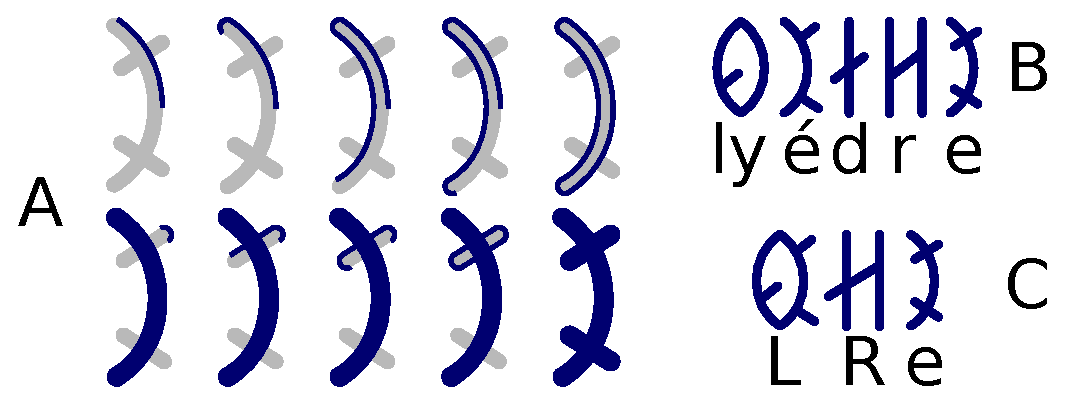
\includegraphics[scale=0.6]{img/w3c_erdely_eps}
    \caption{\label{erdely}
%    \item Az ,,Erdély'' szó \emph{székely
%    írással}~\cite{Saandor:2014:szeekely}. Fent minden graféma külön áll, míg lent összevonva
%    ligatúraképzéssel.
%    \item Sematikusan Az ,,e'' graféma felépítésének
%    folyamata a Path elemeivel. Valamint
%    \end{enumerate}
    }
    \end{figure}
Contextre koncentrál, így a CSS elemeket nem kívánjuk támogatni.
    \begin{wrapfigure}{l}{0.5\textwidth}
    \begin{center}
      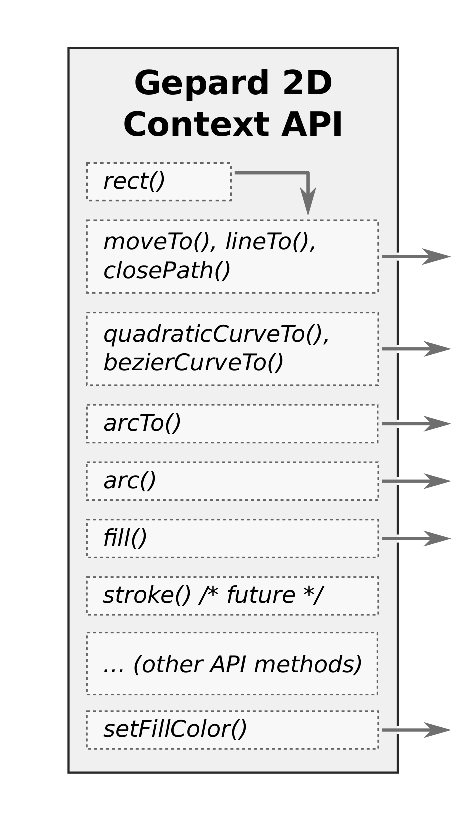
\includegraphics[scale=0.6]{img/dataflow_canvas_api_eps}
    \end{center}
      \caption{\label{dataflow-canvas-API-diagram}
      A Gepard Context 2D API}
    \end{wrapfigure}
Illetve nincs az ábrán a \emph{beginPath} parancs. Végül is az
jelen esetben nem több mint egy törlés és újrakezdés.

  Az ábrán a kimenő nyilak a Gepard belső APIjának a hívásait
jelölik. A \emph{rect} függvény esetében ez nem igényel többet
mint egy megfelelő \emph{moveTo}, három \emph{lineTo} és egy
\emph{closePath} hívást. Azaz visszavezetjük a Canvas 2D már
megvalósított függvényeire.

  Érdemes még néhány szót ejteni a \emph{stroke} hívásról is. Ez
a rész a jelen dolgozatnak nem témája. Viszont a jövőben ennek e
résznek a megvalósításakor -- legalábbis első körben -- úgy fogunk
eljárni, hogy visszavezetjük a strokeot a fillre. Lévén, hogy adott
szélességű stroke által lefedett területet felfoghatjuk úgy is mint egy
kitöltéssel rajzolt bonyolultabb alakzatot. Így a strokenak is a fill
lesz a lelke.

    \section[GLES2 API]{Az OpenGL-ES 2.0 API}
    \label{GLES2 API}

  Az OpenGL-ES azaz az OpenGL Embeded System 2.0-ás verziója a
Khronos Group által felügyelt grafikus meghajtó szabvány.

    \section[Matematikai háttér]{Matematikai háttér}
    \label{Matematikai háttér}

  TODO: Matematikai háttér bevezetője

    \subsection{Seprő-egyenesek}
    \label{Seprő-egyenesek}

  TODO: néhány szó az általános adott külső pontból húzott
félegyenesek által

    \subsection{Bézier-görbe és a de Casteljau felbontás}
    \label{Bézier-görbe és a de Casteljau felbontás}

  A

\begin{equation}
%
\mathbf{B}(t)=\sum_{i=0}^{3} B_i(t) \mathbf{b}_i %\nonumber
%\]
\end{equation}

ahol $\mathbf{B}(t)=(x(t), y(t))$ a $t\in[0,1]$ paraméter által

    \subsection{Körívek közelítése Bézier-görbékkel}
    \label{}

%%%%%%%%%%%%%%%%%%%%%%%%%%%%%%%%%%%%%%%%%%%%%%%%%%%%%%%%%%%%%%%%%%%%%%
%%   Path API                                                       %%
%%%%%%%%%%%%%%%%%%%%%%%%%%%%%%%%%%%%%%%%%%%%%%%%%%%%%%%%%%%%%%%%%%%%%%

    \chapter{Belső Path API}

  A \emph{Gepard} tervezésekor fontos szempont volt, hogy ne csak az
GLES2 API-val működjön. Lehetőséget kell kínálni, hogy a jövőben
több grafikus meghajtó közül lehessen választani. Mint például
a Vulkan, DirectX, esetleg egy referencia szoftveres
raszterizáló. Ezért a Gepard külső API-ján
belül terveztünk egy belső API-t, amely már a választott
rendererrel rajzol. A mi esetünkben ez a belső API-nak a Path
része. Ez rajzol GLES2-t használva. Ebben a részben kell elvégezni
azokat az átalakításokat, visszavezetéseket, amelyeket ugyanitt
háromszögek formájában kirajzolunk.

  Ebben a fejezetben fogjuk bemutatni ennek a belső Path API-nak a
felépítését és működését. Elsőnek áttekintve a
felépítését, majd részletezve az egyes megoldásokat és
visszavezetéseket, közelítéseket.

    \section[Felépítése]{Felépítése}
    \label{Felépítése}

    \begin{wrapfigure}{l}{0.5\textwidth}
    \begin{center}
      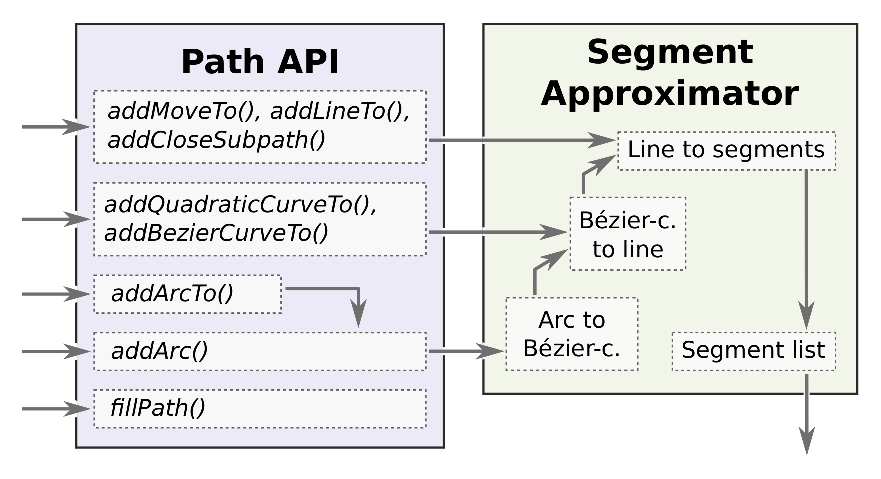
\includegraphics[scale=0.6]{img/dataflow_path_api_eps}
    \end{center}
      \caption{\label{dataflow-path-API-diagram} A belső Path API
      részei és a szakaszokra bontás fázisai}
    \end{wrapfigure}


    \begin{figure}[h]
    \centering
    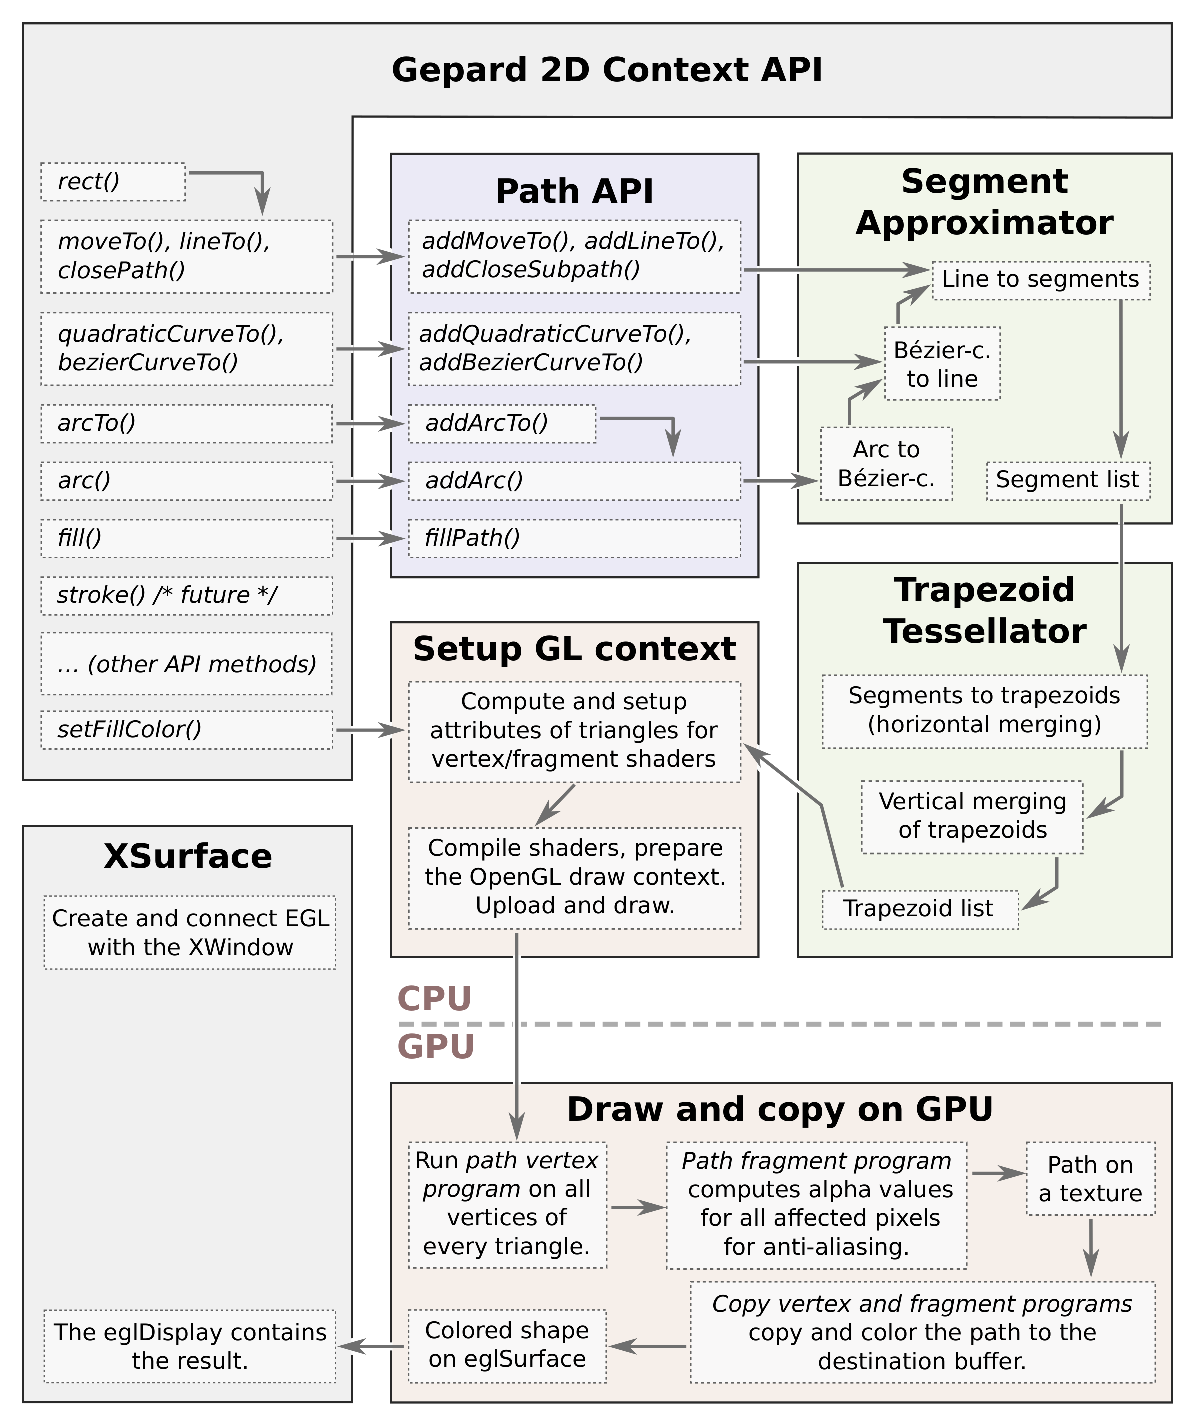
\includegraphics[scale=0.6]{img/dataflow_eps}
    \caption{\label{dataflow-diagram} A rajzolás folyamata}
    \end{figure}


%%%%%%%%%%%%%%%%%%%%%%%%%%%%%%%%%%%%%%%%%%%%%%%%%%%%%%%%%%%%%%%%%%%%%%
%%   Konklúzió                                                      %%
%%%%%%%%%%%%%%%%%%%%%%%%%%%%%%%%%%%%%%%%%%%%%%%%%%%%%%%%%%%%%%%%%%%%%%

    \chapter{Konklúzió}
    \addcontentsline{toc}{section}{Konklúzió}


%%%%%%%%%%%%%%%%%%%%%%%%%%%%%%%%%%%%%%%%%%%%%%%%%%%%%%%%%%%%%%%%%%%%%%
%%   Irodalomjegyzék                                                %%
%%%%%%%%%%%%%%%%%%%%%%%%%%%%%%%%%%%%%%%%%%%%%%%%%%%%%%%%%%%%%%%%%%%%%%

    \bibliography{bib/cites}{}
    \bibliographystyle{bib/huplain}

%%%%%%%%%%%%%%%%%%%%%%%%%%%%%%%%%%%%%%%%%%%%%%%%%%%%%%%%%%%%%%%%%%%%%%
%%   Nyilatkozat                                                    %%
%%%%%%%%%%%%%%%%%%%%%%%%%%%%%%%%%%%%%%%%%%%%%%%%%%%%%%%%%%%%%%%%%%%%%%

    \chapter*{Nyilatkozat}
    %Egy üres sort adunk a tartalomjegyzékhez:
    \addtocontents{toc}{\ }
    \addcontentsline{toc}{section}{Nyilatkozat}
    %\hspace{\parindent}

    % A nyilatkozat szövege más titkos és nem titkos dolgozatok esetében.
    % Csak az egyik típusú nyilatkozatnak kell a dolgozatban szerepelni
    % A pontok helyére az adatok értelemszerűen behelyettesítendők és
    % a szakdolgozat /diplomamunka szó megfelelően kiválasztandó.


    % A nyilatkozat szövege TITKOSNAK NEM MINŐSÍTETT dolgozatban a következő:
    % A pontokkal jelölt szövegrészek értelemszerűen a szövegszerkesztőben és
    % nem kézzel helyettesítendők:

    \noindent

Alulírott \makebox[4cm]{\dotfill} szakos hallgató, kijelentem, hogy a dolgozatomat a Szegedi Tudományegyetem, Informatikai Tanszékcsoport \makebox[4cm]{\dotfill} Tanszékén készítettem, \makebox[4cm]{\dotfill} diploma megszerzése érdekében.

Kijelentem, hogy a dolgozatot más szakon korábban nem védtem meg, saját munkám eredménye, és csak a hivatkozott forrásokat (szakirodalom, eszközök, stb.) használtam fel.

Tudomásul veszem, hogy szakdolgozatomat / diplomamunkámat a Szegedi Tudományegyetem Informatikai Tanszékcsoport könyvtárában, a helyben olvasható könyvek között helyezik el.

    \vspace*{2cm}

    \begin{tabular}{lc}
    Szeged, \today\
    \hspace{2cm} & \makebox[6cm]{\dotfill} \\
    & aláírás \\
    \end{tabular}


%%%%%%%%%%%%%%%%%%%%%%%%%%%%%%%%%%%%%%%%%%%%%%%%%%%%%%%%%%%%%%%%%%%%%%
%%   Köszönetnyilvánítás                                            %%
%%%%%%%%%%%%%%%%%%%%%%%%%%%%%%%%%%%%%%%%%%%%%%%%%%%%%%%%%%%%%%%%%%%%%%

    \chapter*{Köszönetnyilvánítás}
    \addcontentsline{toc}{section}{Köszönetnyilvánítás}

Ezúton szeretnék köszönetet mondani \textbf{X. Y-nak} ezért és ezért \ldots


\end{document}
